%-------------------------------------------------------------------------------
\section{Problem}\label{s:problem}
%-------------------------------------------------------------------------------

The problem that leads to the spike in latencies is that Linux will run a BE
process on one core, unaware that an LC process is runnable and waiting on
another (\autoref{ss:mechanistic}). This observation points to a problem with
the \cgroups{} weight interface: it is expensive to enforce weights across cores
(\autoref{ss:cross-core-hard}). However, even if implemented correctly, the
\cgroups{} weight interface is not well-suited for isolating LC from BE, because
weights interact with sheduling quanta in bad ways: the scheduler can't help but
run the BE processes for a whole quantum when it's weight does accrue, leaving
LC processes interrupted for 4 ms at a time (\autoref{ss:quantum}). We conclude
that the weight-based interface is not well-suited to isolate LC from BE.

\subsection{The mechanistic problem}\label{ss:problem:mechanistic}

\begin{figure}[t]
    \centering
    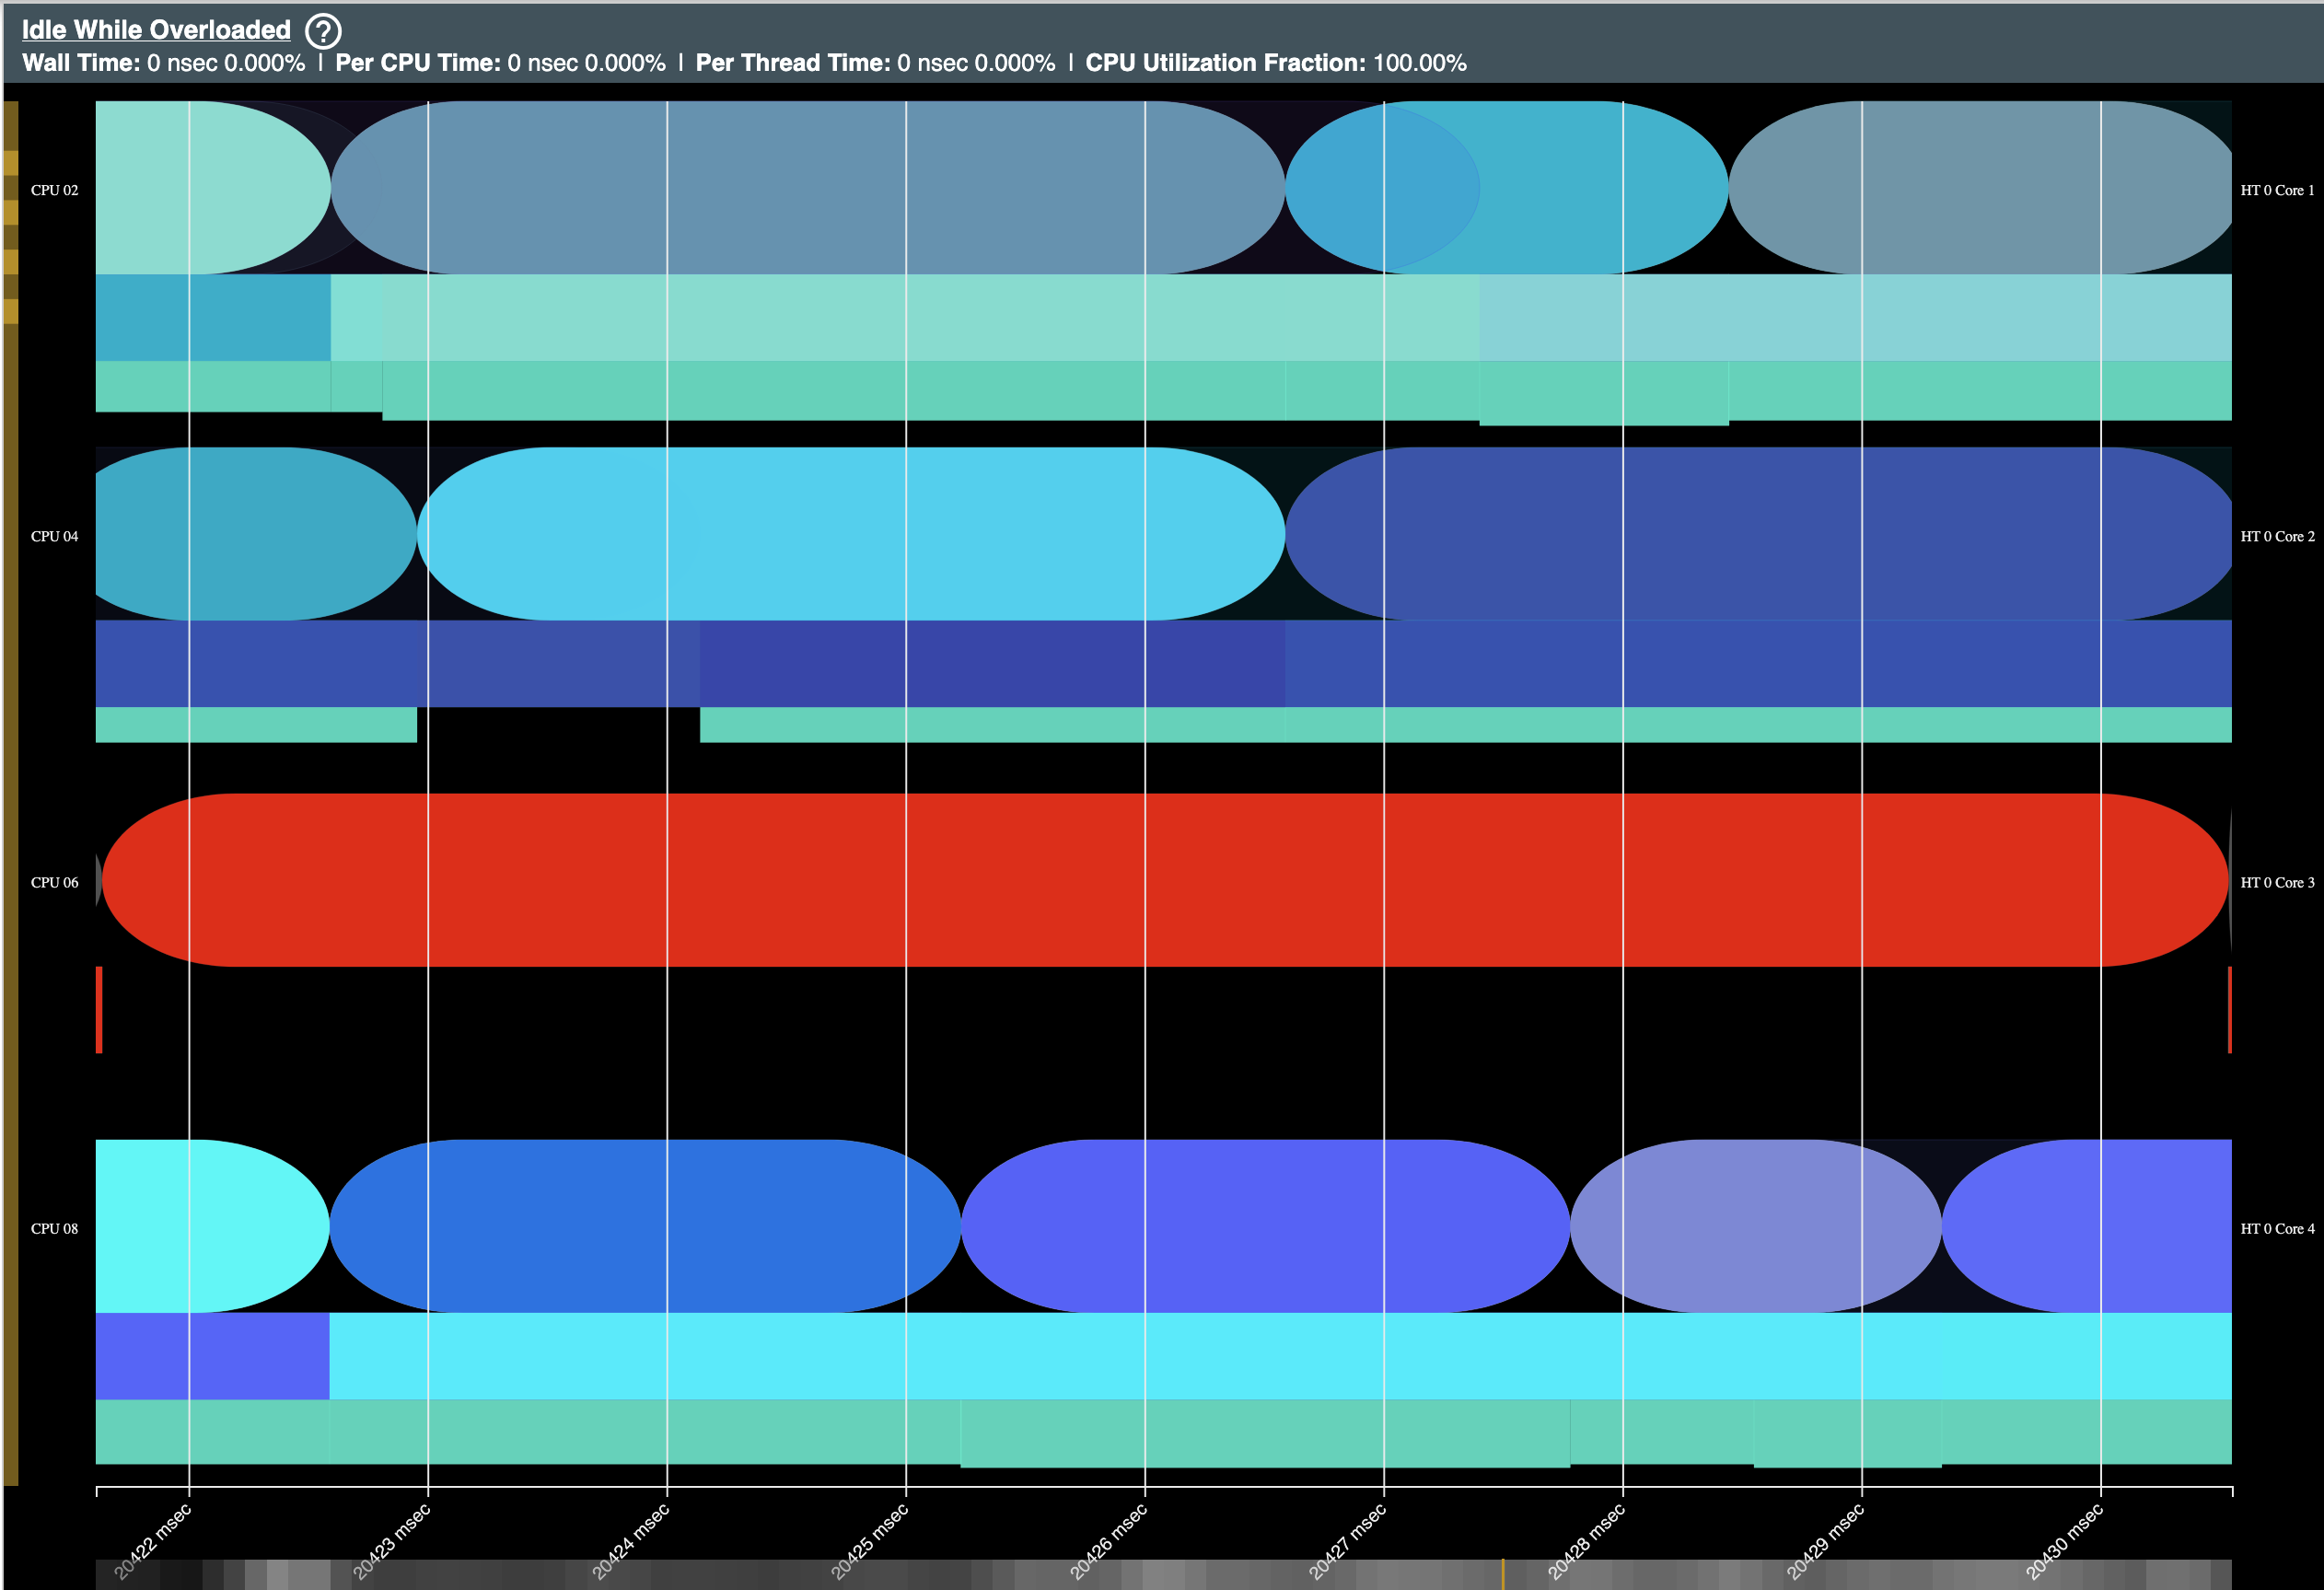
\includegraphics[width=\columnwidth]{graphs/schedviz-problem.png}
    \caption{Each thread is a different color. Circles represent which
    thread is running on that core, while rectangles underneath show waiting but
    runnable threads
    }\label{fig:schedviz-problem}
\end{figure}

The failure mode we observe is that \textit{one core is running a BE process,
while an LC process is waiting on another}. We analyze perf traces of the
scheduling decisions, and visualize the trace using schedviz~\cite{TODO}.
\autoref{fig:schedviz-problem} shows a 10ms outtake of the resulting image. The
process running on each core is shown as a an oval, and queued processes are
shown as rectangles below. The root of the undesirable behavior is: on core 6,
the red process that is running the whole time is a BE process, whereas LC
threads, shown in varying shades of blue, are queued on the other cores.

The reason this happens is that Linux maintains a separate runqueue on each
core, in order to avoid the synchronization overheads of accessing global state
for every scheduling decision. Within each runqueue, Linux's scheduler works to maintain the
correct ratio of received cputime at each scheduling; but Linux does not enforce
the weight ratios across cores. This leads to the above failure mode, where one
core has no runnable high weight processes and thus runs a low weight one,
whereas another core has queued high weight processes. This problem goes away
when there are no BE processes, because cores try to steal work before going
idle.

\subsection{Enforcing weights across cores is
expensive}\label{ss:problem:cross-core-hard}

The root of the problem goes deeper than just a poor implementation: a
weight-based interface is at odds with machine-wide policy enforcement. In
increasingly multi-core and multi-NUMA machines, synchronization is expensive.
This means that the overheads of maintaining global invariants can quickly
become prohibitive.

In order to strictly and globally enforce a processes weight, the scheduler
would need to synchronize at every scheduling decision: calculating whether a
given process is owed time globally requires knowing the total weight across all
cores as well as the sum of time that all the processes in the group have
gotten. At the same time, servers now have up to 8 NUMA nodes, and hundreds up
CPUs across them~\cite{TODO}. Synchronizing across them is expensive: in a
microbenchmark we found that even on a single NUMA node if each core takes a
lock to read the state of the rq on the other cores at every scheduling, this
can take between 10 and 20 $\mu$s. Other work has also found that kernel lock
contention is a bottleneck to performance at scale~\cite{TODO}
% \hmng{the AFaaS cgroups pool thing}


\subsection{Weights interact poorly with tick-based
scheduling}\label{ss:problem:quantum}

Even on a single runqueue, using very large weight differentials as an interface
to isolate LC and BE doesn't work well because preemption is tick-based. In a
weight based scheme, BE processes also get a fair share of the CPU. The problem
is that, when this happens, the BE process will interrupt any running LC process
for a whole tick. In Linux, hardware ticks are 4ms long. This means that an LC
thread processing a request may be interrupted for up to 4ms, provided the BE
process runs for that long before blocking. 4ms can be a large amount of for
microservice workloads, whose SLOs are often in the low double digit or even
single digit ms realm.~\cite{TODO}



